\section{Case study}
\label{sect:case-study} %
%%%%%%%%%%%%%%%%%%%%%%%%%%%%%%%%%%%%

In this section, we present a relatively complex case study, named ProcessMan (process management). The aim is to investigate how our proposed software development method is applied to develop software for a real-world problem domain. A key objective is to construct a process model of AGL from both structural and behavioral aspects that are sufficiently expressive for the domain requirements. As an educational institution, the core processes are teaching subjects (a.k.a course modules) to students every semester and formally assessing the students’ performances. Conceptually, a process is a sequence of tasks, each of which is a sequence of actions. A process is created once, by an organization unit, and is periodically applied to the same unit and possibly to other organizational units that have similar needs. For certain processes, task and action would need to be specialized in order to specify more details
Figure~\ref{fig:case-study} shows the domain model that expresses the ProcessMan’s requirements. The model consists of four domain modules. As shown in the figure, the domain module process structure consists of three domain classes (Process, Task, Action) that together describe the general structure of a process, and two other domain classes (Task4Subject, Action4Subject) that describe a specialized structure for the teaching and assessment processes. Task4Subject specializes Task, while Action4Subject specializes Action. The reason that we only specialize Task and Action and not Process is because class Process suffices for use as a common abstraction for all types of processes. At the process level, there is no real distinction between the processes.

\begin{figure*}[ht]
	\centering
	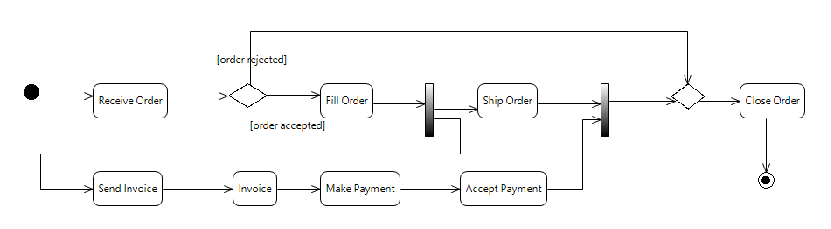
\includegraphics[scale=0.8]{case-study}
	\caption{the model execution of process management} %
	\label{fig:case-study}
\end{figure*}
